\documentclass[a4paper,11pt, floatperchapter]{book}

\usepackage{alphabeta} 
\usepackage{enumitem} 
\usepackage{mathtools}
\usepackage{amsmath, amssymb} 
\usepackage{amsthm}
\usepackage{cancel} 
\usepackage[margin=0.70in]{geometry} 
\geometry{left=2.1cm,right=2.1cm,top=2.4cm,bottom=2.4cm}	%the p1age geometry as defined, A4=210x297mm
\usepackage{graphicx}
\usepackage{wrapfig}
\usepackage[center]{caption}
\usepackage{textcomp}
\usepackage[export]{adjustbox}
\usepackage{tabto}
\usepackage{layout}
\usepackage{bm}
\usepackage{minipage-marginpar}
\usepackage[dvipsnames]{xcolor}
\usepackage{hyperref}
\usepackage{dutchcal}
\usepackage{derivative}
\usepackage{esint}
\usepackage{subcaption}
\usepackage{caption}
\usepackage{fancyhdr}
\usepackage{booktabs}
\usepackage{derivative}
\usepackage{braket}
\usepackage[flushleft]{threeparttable}
\usepackage{float}
%\usepackage[capbesideposition=outside,capbesidesep=quad]{floatrow}
\usepackage{derivative}
\usepackage[thinc]{esdiff}
\usepackage{lipsum}
\usepackage{arydshln}
\usepackage{titlesec}
%\usepackage[style=numeric]{biblatex}
\usepackage[nottoc,notlot,notlof]{tocbibind}
\usepackage[square,numbers,super]{natbib}


\bibliographystyle{abbrvnat}



%%RENEW

\newtheorem{problem}{Άσκηση}
\newtheorem*{solution*}{Λύση}
\newtheorem{definition}{Ορισμός}[subsection]
\newtheorem{properties}{Ιδιότητες}[subsection]
\newtheorem{theorem}{Θεώρημα}[subsection]
\newtheorem{protash}{Πρόταση}[subsection]
\newtheorem{porisma}{Πόρισμα}[subsection]
\newtheorem{lemma}{Λήμμα}[subsection]
\newtheorem*{prooof}{Απόδειξη}
\newtheorem*{notes}{Παρατηρήσεις}
\newtheorem*{note}{Παρατήρηση}
\newtheorem*{app}{Εφαρμογή} 
\newtheorem*{example}{Παράδειγμα}
\newtheorem*{examples}{Παραδείγματα}


\newcommand\numberthis{\addtocounter{equation}{1}\tag{\theequation}}
%\renewcommand{\labelenumi}{\roman{enumi}}
\newcommand{\approxtext}[1]{\ensuremath{\stackrel{\text{#1}}{\approx}}}
%\renewcommand{\tablename}{Πίνακας.}
%\renewcommand\refname{New References Header}
%\renewcommand*\contentsname{Περιεχόμενα}
%\DeclareDerivative{\odv}{\mathrm{d}}



\title{Study of a non-Autonomous Hamiltonian with Canonical Perturbation Theory}
\author{Θωμόπουλος Σπυρίδων}

\titleformat{\chapter}[hang]{\normalfont\huge\bfseries\color{black}}{\thechapter}{1cm}{}{}
%
\newcommand{\changefont}{%
    \fontsize{9}{11}\selectfont
}
\fancyhf{}
\fancyhead[LE,RO]{\changefont \slshape \rightmark} %section
\fancyhead[RE,LO]{\changefont \slshape \leftmark} %chapter
\fancyfoot[C]{\changefont \thepage} %footer
\pagestyle{fancy}
%\fancyhead[L]{\fontsize{10}{12} \selectfont Personal Statement}
%\fancyhead{}
\fancyfoot{}
\fancyfoot[CE,CO]{\thepage}


%\addbibresource{bibliogr.bib}
%\bibliographystyle{dinat}
%\bibliography{bibliogr}

\def\changemargin#1#2{\list{}{\rightmargin#2\leftmargin#1}\item[]}
\let\endchangemargin=\endlist

%========= no-numbers
\setcounter{secnumdepth}{0}
\setcounter{chapter}{0}
%==============

\begin{document}
\begin{titlepage}




\newcommand{\HRule}{\rule{\linewidth}{0.5mm}}

\includegraphics[width=8cm]{Front_Page/logo1.png}\\[1cm] 
\center 
\quad\\[1.5cm]
\textsl{\Large Εθνικό Μετσόβιο Πολυτεχνείο}\\[0.5cm] 
\textsl{\large Σχολή Εφαρμοσμένων Μαθηματικών και Φυσικών Επιστημών}\\[0.5cm] 
\makeatletter
\HRule \\[0.4cm]
{ \huge \bfseries \@title}\\[0.4cm] 
\HRule \\[1.5cm]
\begin{minipage}{0.4\textwidth}
\begin{flushleft} \large
%\emph{Author:}\\
\@author, ge19042
\end{flushleft}
\end{minipage}
~
\begin{minipage}{0.4\textwidth}
\begin{flushright} \large
\emph{Επιβλέπων:} \\
\textup{Γεώργιος Τσιπολίτης}
\end{flushright}
\end{minipage}\\[3cm]
\makeatother
%{\large An Assignment submitted for the UoS:}\\[0.5cm]
{\large \emph{Τεχνολογία Ανιχνευτικών και Επιταχυντικών Διατάξεων}}\\[0.5cm]
%{\large \today}\\[2cm] 
{\large 04 Δεκεμβρίου, 2022}
\vfill 



\end{titlepage}
	



\tableofcontents
\begin{changemargin}{2cm}{2cm} 
\vspace{10cm}
	\section*{Σχόλιο} 
%		This project was done as part of the class "Complex Dynamics of Hamiltonian Systems \& Applications" and it it about the study of a nearly non-integrable Hamiltonian 
%		using Canonical Perturbation Theory.  At first, I study it analytically and then I use Poincare sections in order to study it numerically.
	Αρχικά προσπάθησα να χρησιμοποιήσω fortran για να πάρω τις τομές Poincare, αλλά εν τέλει χρησιμοποίησα την ode45 της matlab καθώς έδινε πολύ πιό γρήγορα τα αποτελέσματα. Oι κώδικες βρίσκονται στην σελίδα \url{https://github.com/spyrosthomo/Physics/tree/main/canonical_perturbation_theory_(In\%20Progress)}
	\let\cleardoublepage\clearpage
\end{changemargin}

\let\cleardoublepage\clearpage

%=========================================================================
%        Theoretical Introduction 
%=========================================================================
\chapter{Theoretical Introduction}
%\addcontentsline{toc}{chapter}{Theoretical Introduction}


Canonical Perturbation Theory (CPT) is the theory which helps us understand how perturbations affect the dynamics of a system which is described from an integrable Hamiltonian. So, if we have a certain Hamiltonian which, after a Canonical Transformation, can be broken into a fully integrable part and a non-integrable parte, we can apply CPT and predict how the latter changes the dynamics of the initial system. 
	\textcolor{red}{MORE ...}

Let's assume that we have an autonomous Hamiltonian $H_0'(\bm{q},\bm{p})$ which fully describes a system via the Hamilton's equations of motion 
		\begin{subequations}\label{eq1}
			\begin{alignat}{2}
				\dot{q_i} =& \pdv{H_0'(\bm{q},\bm{p})}{p_i}\\
				\dot{p_i} =&-\pdv{H_0'(\bm{q},\bm{p})}{q_i}, i=1,..,n
			\end{alignat}
	\end{subequations}
		
		
 	If we can apply a Canonical Transformation on it which maintains the Hamiltonian character of the system, then we call it a Canonical Transformation. 
 	Let's further assume that there are as many constants of motion as degrees of freedom, 2n. This means that exists a Canonical Transformation, $(\bm{q},\bm{p})\rightarrow (\bm{J},\bm{\theta})$, which makes the new generalized position ignorable. That is, the transformed Hamiltonian is not dependent on it, thus $H_0 = H_0(\bm{J})$. These new Canonical Variables are called \textit{Action-Angle Variables}. The system can now be written as 
 	\begin{subequations}\label{eq2}
		\begin{alignat}{2} 
			\dot{\theta_i} =& \pdv{H_0(\bm{J})}{J_i} \\ 
			\dot{J_i}      =&-\pdv{H_0(\bm{J})}{\theta_i}, i=1,..,n
		\end{alignat} 
	\end{subequations}
	
	From the second equation we can easily obtain that the \textit{Action} is constant for all degrees of freedom, $J_i =\alpha_i$. \textcolor{red}{From the first, we can deduce the the derivative of the \textit{Angle} is constant,} thus the solution of the system is 
	\begin{subequations}\label{eq3}
		\begin{alignat}{2}
			\theta_i =& \omega_{0,i} \cdot t + \theta_0 \\ 
			J_i      =& \alpha_i
		\end{alignat}
	\end{subequations}
 	where $\omega_{0,i} = \partial(H_0(\bm{J})/\partial{J_i}$	
	Now, we can see that the new variable $\bm{\theta}$ is named \textit{Angle} on purpose since, from equation (1a), it can be interpreted as a periodic phase with different frequency for each degree of freedom ´$\bm{\omega} = (\omega_{0,1},..,\omega_{o,n})$.
	If we transform back to the initial variables $(\bm{J},\bm{\theta})\rightarrow(\bm{q},\bm{p})$ we have the solution of the initial system.
	
	However convenient it seems, the above case is, firstly extremely rare and secondly extremely sensitive. Say for example that the Hamiltonian models a real mechanical system. That system is naturally prone to imperfections which will destroy its integrable character and as a result we will not be able to apply the above method of Canonical Transformation to Action-Angle variables in order to find the solution. Or we may want to increase our system's energy, so we have to impose an external periodic stimulation.
	All these doesn't mean that we are unable to study the new \textit{perturbed} system.
	
	The new system is now described by a Hamiltonian $H'(\bm{q},\bm{p},t)$. Due to the fact that it deviates only a little from the initial one, it can be written as 
		\begin{equation}\label{eq4}
			H'(\bm{q},\bm{p},t) = H_0'(\bm{q},\bm{p}) + \epsilon H_1'(\bm{q},\bm{p},t) 
		\end{equation}
	
	Where, $H_0'$ is our integrable Hamiltonian and $H_1'$ is the non-integrable perturbation. So, if we apply the same Canonical Transformation as before, the new Hamiltonian, H, can be written as 
		\begin{equation}\label{eq5}
			H(\bm{J},\bm{\theta},t) = H_0(\bm{J}) + \epsilon H_1(\bm{J},\bm{\theta},t)
		\end{equation}
	
	Our goal now is to transform the new Hamiltonian in order to push the $\bm{\theta},t$ dependence to higher order $\epsilon ^2$. In that way, we will have an approximately integrable Hamiltonian to the first order and we will be able to solve it. 
	
	\section{Canonical Transformation}
	
	The aforementioned transformation, $(\bm{J},\bm{\theta})\rightarrow(\bm{\bar{J}},\bm{\bar{\theta}})$ should as well maintain the Hamiltonian structure of our system, so that the new variables $(\bm{\bar{J}},\bm{\bar{\theta}})$ are Canonical Variables.
	
	The new Hamiltonian is $\bar{H} = \bar{H}(\bm{\bar{J}},\bm{\bar{\theta}})$. Both the new and the old Hamiltonians should obey the Hamilton's variational principle 
	\begin{align}\label{eq6}
		\left\{
		\begin{matrix}
				\delta\int_{t_1}^{t_2}\left( J_i \dot{\theta_i} - H(\bm{J},\bm{\theta},t)\right)dt =& 0\\
				 \delta\int_{t_1}^{t_2}\left( \bar{J}_i \dot{\bar{\theta}}_i - \bar{H}(\bm{\bar{J}},\bm{\bar{\theta}},t)\right)dt =& 0
		\end{matrix}  \right\}\Rightarrow \nonumber \\
		J_i \dot{\theta}_i - H(\bm{J},\bm{\theta},t) =\bar{J}_i \dot{\bar{\theta}}_i - \bar{H}(\bm{\bar{J}},\bm{\bar{\theta}},t) + \odv{F(\bm{J},\bm{\theta},\bm{\bar{J}},\bm{\bar{\theta}},t)}{t} 
	\end{align}
	
	The F function is called as the \textit{Generating Function} of the transformation. That means that it uniquely defines the transformation. Say that we want it to be dependent only on the old Angles and the new Actions,$F(\bm{\theta},\bm{\bar{J}},t)$. Our goal is to solve (\ref{eq6}) for the other two variables, $\bm{\bar{\theta}},\bm{J}$. We have  
	
		\begin{align*}
			J_i\dot{\theta_i}- H(\bm{J},\bm{\theta},t) =\bar{J}_i \dot{\bar{\theta}}_i - \bar{H}(\bm{\bar{J}},\bm{\bar{\theta}},t) + \dot{\theta_i}\pdv{F}{\theta_i} + \dot{\bar{J}}_i\pdv{F}{\bar{J}_i} + \pdv{F}{t}
		\end{align*}
	
	We see that there is no way to get rid of the unwanted term (1st on RHS). For that reason, we have to add one arbitrary term to the generating function which will cancel with the $J_i\dot{\bar{\theta}}_i$. Our generating function will be 
		\begin{align}
			F(\bm{J},\bm{\theta},\bm{\bar{J}},\bm{\bar{\theta}},t) = -\bar{J}_i\bar{\theta}_i + S(\bm{\theta},\bm{\bar{J}},t)
		\end{align}
	
	Now, equation (\ref{eq6}) can be written as 
		\begin{align}
			J_i\dot{\theta_i}- H(\bm{J},\bm{\theta},t) =&\cancel{\bar{J}_i \dot{\bar{\theta}}_i} - \bar{H}(\bm{\bar{J}},\bm{\bar{\theta}},t) + \dot{\theta_i}\pdv{S}{\theta_i} + \dot{\bar{J}}_i\pdv{S}{\bar{J}_i} +\pdv{S}{t} - \dot{\bar{J}}_i\bar{\theta}_i - \cancel{\bar{J}_i\dot{\bar{\theta}}_i } \Rightarrow \nonumber\\
			%
			\textcolor{red}{J_i\dot{\theta_i}}- \textcolor{blue}{H(\bm{J},\bm{\theta},t)} =	&- \textcolor{blue}{\bar{H}(\bm{\bar{J}},\bm{\bar{\theta}},t)} +  \textcolor{red}{\dot{\theta_i}\pdv{S}{\theta_i}} + 			\textcolor{green}{\dot{\bar{J}}_i\pdv{S}{\bar{J}_i}} + \textcolor{blue}{\pdv{S}{t}} - \textcolor{green}{\dot{\bar{J}}_i\bar{\theta}_i} \Rightarrow \nonumber\\ 
%
		\end{align}				
	So we obatin 
	\begin{subequations}\label{eq9}
			\begin{alignat}{3}
							J_i            =& \partial{S}/\partial{\theta_i}
							\vspace{0.4cm} \\ \vspace{0.4cm} 
							\bar{\theta}_i =& \partial{S}/\partial{\bar{J}_i}\\
							\bar{H}        =& H + \partial{S}/\partial{t}
			\end{alignat}
	\end{subequations}			
	So now we know how each variable can be obtained by the generating function $S=S(\bm{\theta},\bar{\bm{J}},t)$. It is clear that S uniquely defines the transformation and if it is equal to $S = \theta_i\bar{J}_i$, it represents the \textit{identity transformation}, since it leaves both $\bm{J}$ and $\bm{\theta}$ unchanged.
	\section{Time Dependent Perturbation Theory}
	
		We want to study a system described by (\ref{eq5}). An integrable system $H_0$ plus an non-integrable one $H_1$ which acts as a perturbation on the first. More specificaly, what we want to do is to move the $\bm{\bar{\theta}}$ dependence of $\bar{H_1}$, to higher order utilizing a Canonical Transformation $(\bm{J},\bm{\theta})\rightarrow (\bm{\bar{J}}, \bm{\bar{\theta}})$. 
		
		Since the non-integrable part is a perturbation, we can deduce that the generating function of the wanted trasformation will be nearly identical, with a non-identical first order part: 
		\begin{align}\label{eq10}
			S(\bm{\theta},\bm{\bar{J}},t) = \bar{J}_i\theta_i + \epsilon S_1(\bm{\theta},\bar{\bm{J}},t) 
		\end{align}
	%
		From (\ref{eq9}) we have 
			\begin{subequations}\label{eq11}
					\begin{alignat}{3}
						J_i  =& \bar{J}_i + \epsilon\pdv{S_1}{\theta_i} \\ 
			  \bar{\theta}_i =& \theta_i + \epsilon\pdv{S_1}{\bar{J}_i} \\  	  \bar{H}(\bm{\bar{J}},\bm{\bar{\theta}},t) =& H(\bm{J},\bm{\theta},t) + \epsilon\pdv{S_1}{t}
					\end{alignat}
			\end{subequations}	
	So we see that for the zero-th order approximation, the new and the old variables are the same. As for the Hamiltonian, we substitute (\ref{eq11}a), (\ref{eq11}b) into (\ref{eq11}c) and we have
%	\vdots \\
%	\textcolor{red}{ WRITE THE TAYLOR EXPANSION FOR THE HAMILTONIAN AND THEN SEPARATE THE ORDERS AND DERIVE EQNS 12}\\
%	\vdots
	%
	%	:) Taylor 
	%	
	\begin{align*}
		\bar{H}(\bm{\bar{J}},\bm{\bar{\theta}},t) =& H(\bm{J}(\bm{\bar{J}},\bm{\bar{\theta}},t), \bm{\theta}(\bm{\bar{J}},\bm{\bar{\theta}},t),t) + \epsilon \pdv{S_1}{t} \xRightarrow{(\ref{eq11}a,b)} \\ 
		=& H_0(\bm{J}(\bm{\bar{J}},\bm{\bar{\theta}},t)) + \epsilon H_1(\bm{J}(\bm{\bar{J}},\bm{\bar{\theta}},t), \bm{\theta}(\bm{\bar{J}},\bm{\bar{\theta}},t),t)  \epsilon+\pdv{S_1}{t} \xRightarrow{(\ref{eq11}a)}\\
		 =&  H_0\left(\bm{\bar{J}} + \epsilon\pdv{S_1}{\bm{\theta}}\right) + \epsilon H_1(\bm{J}(\bm{\bar{J}},\bm{\bar{\theta}},t), \bm{\theta}(\bm{\bar{J}},\bm{\bar{\theta}},t),t)  +\epsilon\pdv{S_1}{t} \xRightarrow{Taylor, up\hspace{0.1cm}to\hspace{0.1cm} (\epsilon^1)}\\  			
		 =& H_0(\bm{\bar{J}}) + \epsilon \pdv{S_1}{\bm{\theta}} \pdv{H_0(\bm{\bar{J}})}{\bm{\bar{J}}} + \epsilon H_1(\bm{\bar{J}},\bm{\bar{\theta}},t) +\epsilon \pdv{S_1}{t}
	\end{align*}		
	%
	So, if we separate the above equation into $0^{th}$ and $1^{st}$ orders, we have
	
	\begin{subequations}\label{eq12}
			\begin{alignat}{3}
				(\epsilon^0):\hspace{0.5cm} \bar{H}_0 =&  \bar{H_0}(\bm{\bar{J}}) = H_0(\bm{\bar{J}}) \\ 
				(\epsilon^1):\hspace{0.5cm} \bar{H}_1 =&  \bar{H_1}(\bm{\bar{J}},\bm{\bar{\theta}},t)  \Rightarrow \nonumber \\
					=& H_1(\bar{\bm{J}}, \bar{\bm{\theta}}, t) + \pdv{S_1}{\bm{\theta}}\cdot \bm{\omega_0}(\bm{\bar{J}})+ \pdv{S_1}{t}
			\end{alignat}
	\end{subequations}	
	%
	Where 
		\begin{align}\label{eq13}
			\bm{\omega_0}(\bm{\bar{J}}) = \pdv{H_0(\bm{\bar{J}})}{\bm{\bar{J}}}
		\end{align}
	Now we have to find which $S_1$ suits us to continue our study, since it defines uniquely the transformation. First of all, if we identify $\bm{\theta}$ as a phase, then $H_1$ has to be a periodic function with respect to $\bm{\theta}$ with period5 $T_{\theta_i} = 2\pi$. We also want time periodicity, with period $T_t = 2\pi/\Omega$.% If the perturbation was not periodic, and say
	%
	Since both $H_1$ and $\bar{H_1}$ are periodic with respect to both \textit{Angle} and \textit{time}, from equation (\ref{eq12}b) we have that $S_1$ should also be a periodic function of \textit{Angle} and \textit{time}
	
	Until now, we have two solid points from which we can continue. Firstly, the periodicity of $H_1$ and $S_1$ and secondly, the fact that we know how to solve integrable systems (with \textit{Angle and time} independent Hamiltonian).
	The above points lead respectively to the Fourier expansion of $H_1$ and $S_1$ and the need to make $\bar{H_1}$ \textit{approximately integrable} (if we could make it exactly integrable we wouldn't need CPT :) ). 	
	The latter requires a subtle, yet extremely useful trick which will lead to the choice of $S_1$ by connecting it with $H_1$. 
	
	To be more specific, the trick is as simple as separating $H_1$ into two parts;a mean value with respect to both \textit{Angle and time} plus an oscillating part
	\begin{equation}\label{eq14}
		H_1 = \langle H_1 \rangle_{\bm{\bar{\theta}}, t} + \{H_1\}_{\bm{\bar{\theta}}, t} 
	\end{equation}
	%
Now, if we substitute into (\ref{eq12}b) we have 
	\begin{align}\label{eq15}
		 \bar{H_1} =& H_1(\bar{\bm{J}}, \bar{\bm{\theta}}, t) + \pdv{S_1}{\bm{\theta}}\cdot \bm{\omega_0}(\bm{\bar{J}})+ \pdv{S_1}{t} \Rightarrow\nonumber\\
		  		  =& \langle H_1 \rangle_{\bm{\bar{\theta}}, t}(\bar{\bm{J}}) + \{H_1\}_{\bm{\bar{\theta}}, t}(\bar{\bm{J}}, \bar{\bm{\theta}}, t) + \pdv{S_1}{\bm{\theta}}\cdot \bm{\omega_0}(\bm{\bar{J}})+ \pdv{S_1}{t}
	\end{align}
	
	Here is the crucial point where we will \textit{"push"} the $\bm{\theta}-t$ dependence to higher orders and at the same time we define the Canonical Transformation by defining its gerating function $S_1$. Since we can arbitrarily choose $S_1$, we choose it in order to satisfy the following relation
	\begin{equation}\label{eq16}
		\{H_1\}_{\bm{\bar{\theta}}, t}(\bar{\bm{J}}, \bar{\bm{\theta}}, t) + \pdv{S_1}{\bm{\theta}}\cdot \bm{\omega_0}(\bm{\bar{J}})+ \pdv{S_1}{t} = 0
	\end{equation}	
We finally have that 
	\begin{align}\label{eq17}
		\bar{H} =&  \bar{H_0} + \epsilon\bar{H_1}  \Rightarrow\nonumber\\
				=& H_0(\bar{\bm{J}}) + \epsilon\langle H_1 \rangle_{\bm{\bar{\theta}}, t}(\bar{\bm{J}}) 
	\end{align}
which is dependent (approximately) only on $\bar{\bm{J}}$ and is an integrable (approximately) Hamiltonian.

There is only one step left to complete the theory. That is to determine $S_1$ by writing it as a Fourier sum and obtaining the coefficients from (\ref{eq16}). The Fourier series of $\{H_1\}_{\bm{\bar{\theta}},t}$\footnotemark and $S_1$
	\footnotetext{The function $\{H_1\}_{\bm{\bar{\theta}},t}$ has no constant part as we have taken out of it as a mean value at (\ref{eq14}). This means that we will not start the Fourier sum from 0.}
	
\begin{subequations}\label{eq18}
		\begin{alignat}{2}	
		\{H_1\}_{\bm{\bar{\theta}},t}(\bm{\bar{J}}) =& \sum_{\bm{l},m\neq0}^\infty H_{1,\bm{l},m} \cdot e^{i(\bm{l}\cdot\bm{\theta}+m\Omega t)} \\ 
		S_1                           =& \sum_{\bm{l},m\neq0}^\infty S_{1,\bm{l},m} \cdot e^{i(\bm{l}\cdot\bm{\theta}+m\Omega t)} 
		\end{alignat}
\end{subequations}	
%
We substitute (\ref{eq18}) into (\ref{eq16}) and we have 
	\begin{align}\label{eq19} 
			\sum_{\bm{l},m\neq0}^\infty \left( H_{1,\bm{l},m} \cdot 
			e^{i(\bm{l}\cdot\bm{\theta}+m\Omega t)} + \bm{\omega_0}(\bm{\bar{J}})\cdot i\bm{l} \cdot S_{1,\bm{l},m} \cdot e^{i(\bm{l}\cdot\bm{\theta}+m\Omega t)} +
			im\Omega S_{1,\bm{l},m} \cdot e^{i(\bm{l}\cdot\bm{\theta}+m\Omega t)}\right) =& 0 \Rightarrow \nonumber \\ 
			%
			\sum_{\bm{l},m\neq0}^\infty \left(  H_{1,\bm{l},m} + i\left(\bm{\omega_0}(\bm{\bar{J}})\cdot \bm{l}  + m\Omega\right)\cdot S_{1,\bm{l},m}  
					\right)e^{i(\bm{l}\cdot\bm{\theta}+m\Omega t)} =& 0  \xRightarrow{\forall\hspace{0.05cm}\bm{l},m\neq0} \nonumber \\
			\hspace{-2cm}S_{1,\bm{l},m} =  i\frac{H_{1,\bm{l},m}}{\bm{\omega_0}(\bm{\bar{J}})\cdot \bm{l} + m\Omega}&
	\end{align}
%
where $H_1$ may act as a perturbation whether $V_1,V_2<<1$.

Now, the transformation which "pushes" the \textit{Angle} dependence of $\bar{H_1}$ is fully defined by equations (\ref{eq18}b) and (\ref{eq19}) and our job is just to find the Fourier coefficients of $H_1$.
	\begin{equation}\label{eq20}
		S_1 = \sum_{\bm{l},m\neq0}^\infty i\frac{H_{1,\bm{l},m}(\bar{\bm{J}})}{\bm{\omega_0}(\bm{\bar{J}})\cdot \bm{l} + m\Omega} \cdot e^{i(\bm{l}\cdot\bm{\theta}+m\Omega t)} 
	\end{equation}

\section{Final Remarks}
From the above equation we can see that there may exist certain values of $\bm{l}$ and m, for which the denominator becomes zero
	\begin{equation}\label{eq21}
		\bm{\omega_0}(\bm{\bar{J}})\cdot \bm{l} + m\Omega = 0
	\end{equation}
This means that the perturbation is no longer a perturbation since it has huge values compared to the integrable part and we have a huge problem.  

If we had only the integrable part, then the dynamics of the systems evolve on a n-dimensional torus with the constant \textit{Action} being the radius and the linearly increasing \textit{Angle} being the phase. 
	There are two cases, which depend on the frequency (time derivative of the \textit{Angle}) of each degree of freedom. If the ratio of each two frequencies is a \textbf{rational} number, $\omega_i/\omega_j \in\mathbb{Q},\forall i,j$, then the motion is periodic and the trajectory does not fill the the whole "surface" of the torus. 
	On the other hand, if the ratio is \textbf{irrational} even for one pair of frequencies, $\exists i,j: \omega_i/\omega_j\in\mathbb{R}/\mathbb{Q}$, the motion is not periodic and the trajectory densly fills the surface of the torus.
	
	This behaviour is easily shown with Poincare Maps. To make a Poincare Map we firstly construct a surface on the phase space in which we choose some degrees of freedom to be constant (in our case some \textit{Angles}) and we as we let the system evolve, we see where the trajectory intersects our surface. If we are in the first case of a periodic system, we will see points which will repeat after one period, whereas if we are the second case of irrational ratios, we will see dense regions of points.  
		\begin{figure}[h!]
			\centering 
			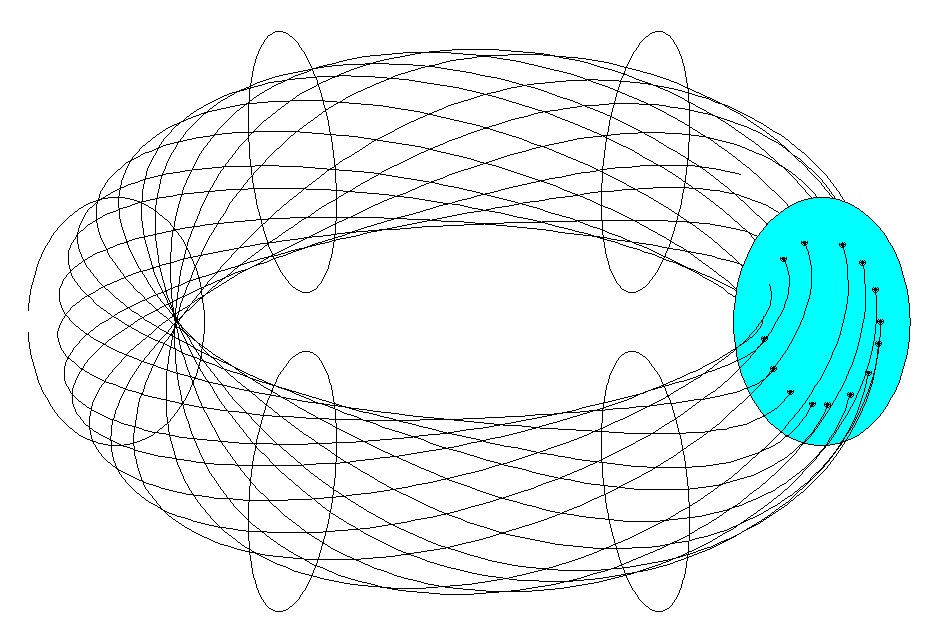
\includegraphics[scale=0.3]{Theory/poin.png}
			\caption{Poincare Diagram of a 2D periodic system}
			\label{fig1}
		\end{figure}
		
	These were about the integrable system. If we turn on the non-integrable part,
%=========================================================================
%        Hamiltonian - 1 
\chapter{Non-autonomous Hamiltonian }
%\addcontentsline{toc}{chapter}{Non-autonomous Hamiltonian }
We will use the theory developed in the above text for systems with n degrees of freedom, in order to study the follwing Hamiltonian with one degree of freedom 
	\begin{equation}\label{eq2.1}
		H(J,\theta,t) = \bar{\omega}J + J^k + V_1cos(n_1\theta-m_1\Omega t) + V_2cos(n_2\theta-m_2\Omega t)
	\end{equation} 
	%
It is obvious that it can be written as the sum of an integrable and a non-integrable Hamiltonian
	\begin{subequations}\label{eq2.2}
			\begin{alignat}{2}
				H_0 =& \bar{\omega}J + J^k\\
				H_1 =& V_1cos(n_1\theta-m_1\Omega t) + V_2cos(n_2\theta-m_2\Omega t)
			\end{alignat}
	\end{subequations}	
	%
This means that if we "turn off" the non-integrable part by setting $V_1=V_2=0$, we can easily find the frequency from the Hamilton's equation of motion for the generalized position
	\begin{align*}\label{eq2.3}
		\omega_0(J) =& \dot{\theta} = \pdv{H_0}{J} \Rightarrow\\
			     =& \bar{\omega} + k J^{k-1} \numberthis
	\end{align*}
	%
The non integrable part can be written as a sum of mean value and an oscillating part 
	\begin{align*}
		H_1 = \langle H_1 \rangle_{\theta,t} + \{ H_1 \}_{\theta,t}
	\end{align*}
But since it is a periodic function with respect to $\theta, t$, we have 
	\begin{align*}
		\langle H_1 \rangle_{\theta,t} =0
	\end{align*}
and since it is already a sum of cosine functions we will not use the Fourier expansion (\ref{eq18}a) but the following 
	\begin{align}\label{eq2.4}
		\{ H_1 \}_{\theta,t} = H_1 = \sum_{i=1,2} H_{1,i} cos(n_i\theta-m_i\Omega t)
	\end{align}
where 
	\begin{equation}
		H_{1,i} = 
		\begin{cases}
			V_i &, i=1,2\\
			0   &, \text{otherwise}
		\end{cases}
	\end{equation}
Similarly, we write $S_1$ as the following sum
	\begin{align}\label{eq2.6}
		S_1 = \sum_{i} S_{1,i} sin(n_i\theta-m_i\Omega t) 
	\end{align}
If we substitute (\ref{eq2.4}) and (\ref{eq2.6}) into the condition (\ref{eq16}), we have 
	\begin{align*}
		H_1 + \pdv{S_1}{\theta} \omega_0(\bm{\bar{J}})+ \pdv{S_1}{t} = 0 \Rightarrow\\
		%
		\sum_i \left( V_icos(n_i\theta-m_i\Omega t) + m_i\Omega S_{1,i}cos(n_i\theta-m_i\Omega t)  -n_iS_{1,i}cos(n_i\theta-m_i\Omega t)  \cdot \omega_0 \right) = 0 \Rightarrow \\ 
		\sum_i\left( V_i + m_i\Omega S_{1,i}-n_iS_{1,i}\omega_0\right)cos(n_i\theta-m_i\Omega t) =0 \Rightarrow\\ 
	\end{align*}
We want it to hold $\forall i=\{1,2\}$
	\begin{align*}%\label{eq2.7}
		S_{1,i} = \frac{V_i}{-m_i\Omega + n_i(\bar{\omega}+kJ^{k-1})}, i=1,2
	\end{align*}
	%
So, for each term of the expansion, we have resonance for the values for which the denominator is zero 
	\begin{align}\label{eq2.7}
		-m_i\Omega + n_i(\bar{\omega}+kJ^{k-1}) = 0\Rightarrow\nonumber\\
		J_{res,i}^{k-1} =  \frac{m_i\Omega - n_i\bar{\omega}}{kn_i}
	\end{align}
%
%
%
%========================================================================
% Q -3 
%========================================================================
%
%
\textcolor{red}{
\line(1,0){450}\\
\begin{center}
	\textbf{QUESTION 3}
\end{center}
\line(1,0){450}\\
}

Also, we can compute the approximate (up to first order) constant of motion $\bar{J}$ from (\ref{eq11}a)
	\begin{align*}\label{eq2.8}
		\bar{J} =& J - \pdv{S_1}{\theta} \Rightarrow\\ 
		        =& J - \sum_{i=1,2}S_{1,i}n_i cos(n_i\theta-m_i\Omega t)\Rightarrow\\ 
		        =& J - \frac{V_1n_1}{m_1\Omega + n_1(\bar{\omega}+kJ^{k-1})}cos(n_1\theta-m_1\Omega t) -\frac{V_2n_2}{m_2\Omega + n_2(\bar{\omega}+kJ^{k-1})} cos(n_2\theta-m_2\Omega t)\numberthis
	\end{align*}


%===============================================================
%
%
%
\textcolor{red}{
\line(1,0){450}\\
\begin{center}
	\textbf{QUESTION 2}
\end{center}
\line(1,0){450}\\
}
%
%
%========================================================================
% second Q
%========================================================================
%
%
%
If we take either $V_1=0$ or $V_2=0$, then we can change the position variable with the transformation 
	\begin{align}\label{eq2.9}
		\hat{\theta} = n_i\theta-m_i\Omega t, \text{\hspace{.3cm}$i=$1 or 2}
	\end{align}
But if we want to use a Canonical Transformation, we can also choose 
	\begin{align}\label{eq2.10}
		\hat{J} = \alpha J 
	\end{align}
where $\alpha$ is to be determined. In order to demand a Canonical Transformation and by doing so, to find $\alpha$, we can use the \textit{symplectic condition} $\tilde{\bm{M}}\bm{J}\bm{M} = \bm{J}$, where $\bm{M}$ is the Jacobian of the transofrmation, or the \textit{Poisson Bracket Condition}, $[\hat{\theta},\hat{J}]=1$, or directly find a generating function. 

	We will use the \textit{Poisson Bracket Condition} in order to determine $\alpha$ and then we will find the generating function of the transformation.
	If we want the transformation to be Canonical, then the following condtion must hold 
	\begin{align*}\label{eq2.11}
		[\hat{\theta},\hat{J}] =& 1 \Rightarrow\\
		\pdv{\hat{J}}{J}\pdv{\hat{\theta}}{\theta} - \cancel{\pdv{\hat{J}}{\theta}}\cancel{\pdv{\hat{\theta}}{J}} =& 1 \xRightarrow{(\ref{eq2.9}),(\ref{eq2.10})}\\ 
		\alpha n_i =& 1 \Rightarrow\\ 
		\alpha =& 1/n_i , \text{\hspace{.6cm}$i=$1 or 2}   \numberthis
	\end{align*}
%
%
In general, the generating function of the Canonical Transformation can be dependent on any pair of new and old variables. We choose it to be $F_2=F_2(\theta,\hat{J})$. Now, the other two variables, can be expressed with $F_2$. For $\hat{\theta}$ 
	\begin{align*}\label{eq2.12}
		\hat{\theta}          =& \pdv{F_2}{\hat{J}} \xRightarrow{(\ref{eq2.9})}\\ 
		n_i\theta-m_i\Omega t =& \pdv{F_2}{\hat{J}}\xRightarrow{\theta - indep.} \\ 		
		F_2 =& (n_i\theta-m_i\Omega t)\hat{J} + f(\theta)\numberthis
	\end{align*}
And for J
	\begin{align*}
		J  =&\pdv{F_2}{\theta} \xRightarrow{(\ref{eq2.12}),(\ref{eq2.10})} \\ 
n_i\hat{J} =& n_i\hat{J}+f'(\theta) \Rightarrow\\ 
		 f(\theta) =& const.				
	\end{align*}
So, we can ignore $f(\theta)$ since in our transformation it appears only as a derivative. Finally, the generating function is 
	\begin{equation}\label{eq2.13}
		F_2(\theta,\hat{J}) = (n_i\theta - m_i\Omega t)\hat{J}, \text{\hspace{.3cm}$i=$1 or 2}
	\end{equation}
%
The new Hamiltonian, according to (\ref{eq9}c) is 
	\begin{align*}\label{eq2.14}
		\hat{H}(\hat{\theta},\hat{J}) =& H(\hat{\theta}, \hat{J}) + \partial{F_2}/\partial{t} \Rightarrow\\ 
									  =& (\bar{\omega}n_i-m_i\Omega )\hat{J} + n_i^k\hat{J}^k +V_icos\hat{\theta} \numberthis
	\end{align*}
And since it depends on $\hat{\theta}$, it is not integrable, but again, it can been seen as a sum of an integrable and a non-integrable perturbation. So, from CPT and (\ref{eq11}a), the first order approximation of the new \textit{Action}, is 
	\begin{align*}
		\hat{\bar{J}} = \hat{J} - \epsilon\pdv{S_1}{\hat{\theta} }
	\end{align*}
Where $S_1$ is the same as the one we calculated (\ref{eq2.6}) for the full Hamiltonian (both $V_1,V_2\neq0$) without the one sine term, thus 
	\begin{align*}
		\hat{\bar{J}} = \hat{J} - \epsilon\frac{V_i}{m_i\Omega-n_i(\bar{\omega}+k\hat{J}^{k-1})}cos\hat{\theta} , \text{\hspace{.6cm}$i=$1 or 2}   \numberthis
	\end{align*}
	%
	The \textit{resonance Action} can be obtained if we set the above denominator equal to zero
		\begin{align*}\label{eq2.16}
			m_i\Omega-n_i(\bar{\omega}+k\hat{J_{res}}^{k-1})=0 \Rightarrow\\
			\hat{J}_{res}^{k-1} = \frac{m_i\Omega-n_i\bar{\omega}}{n_ik}\numberthis
		\end{align*}
	%
	If we expand our Hamiltonian (\ref{eq2.14}) around $\hat{J}_{res}$, with $\Delta \hat{J} = \hat{J} - \hat{J}_{res}$, we have 
\begin{align}\label{eq2.17}
	\hat{H}\simeq&  \hat{H}(\hat{J}_{res}) + 
					\cancel{\left. \pdv{\hat{H}}{\hat{J}}\right|_{\hat{J}_{res}}}\Delta\hat{J} +
					 \left. \pdv[order=2]{\hat{H}}{\hat{J}}\right|_{\hat{J}_{res}}(\Delta\hat{J})^2 + O(\epsilon^2)\xRightarrow{\pdv{\theta}{t}|_{res}=0=\pdv{\hat{H}}{\hat{J}}|_{res}}\nonumber\\
					 =& \left[(\bar{\omega}n_i-m_i\Omega )\hat{J}_{res} + n_i^k\hat{J}_{res}^k +V_icos\hat{\theta} \right]+ 
					 \frac{1}{2}k(k-1)\hat{J}_{res}(\Delta\hat{J})^2\Rightarrow\nonumber\\
					=& V_i cos\hat{\theta} + \frac{1}{2}k(k-1)\hat{J}_{res}(\Delta\hat{J})^2
						+\underbrace{\left[(\bar{\omega}n_i-m_i\Omega )\hat{J}_{res} + n_i^k\hat{J}_{res}^k \right]}_{constant}
\end{align}

%		\begin{align*}\label{eq2.17}
%			\hat{H}\simeq&  \hat{H}(\hat{J}_{res}) + 
%					\left. \pdv{\hat{H}}{\hat{J}}\right|_{\hat{J}_{res}}(\hat{J}-\hat{J}_{res}) +
%					 \left. \pdv[order=2]{\hat{H}}{\hat{J}}\right|_{\hat{J}_{res}}(\hat{J}-\hat{J}_{res})^2 + O(\epsilon^2)\Rightarrow\\
%	%---------				 
%	% 1st term			
%			=&	\left[(\bar{\omega}n_i-m_i\Omega )\hat{J}_{res} + n_i^k\hat{J}_{res}^k +V_icos\hat{\theta} \right]+ 
%	% 2nd term 
%			   \left[ (\bar{\omega}-m_i\Omega) + kn_i^k\hat{J}_{res}^{k-1}\right]( \hat{J}-\hat{J}_{res}) + \\
%	% 3rd term 
%			&\text{\hspace{2cm}} +\left[  k(k-1)\hat{J}_{res}^{k-1} \right](\hat{J}-\hat{J}_{res})^2 \Rightarrow\\
%			=& \textcolor{red}{n_i^k\hat{J}_{res}^{k}}+V_icos\hat{\theta} +
%			 	\textcolor{green}{(\bar{\omega}n_i-m_i\Omega)\hat{J}}+ 
%			 \textcolor{green}{kn_i^k\hat{J}_{res}^{k-1}\hat{J}}-\textcolor{red}{kn_i^k\hat{J}_{res}^k}
%			+ 1/2k(k-1)n_i^k\hat{J}_{res}^{k-2}\hat{J}^2+\\
%			&\text{\hspace{2cm}} +\textcolor{red}{1/2k(k-1)n_i^k\hat{J}_{res}^k}-\textcolor{green}{k(k-1)n_i^k\hat{J}_{res}^{k-1}\hat{J}}\Rightarrow\\
%			%
%			%
%			=& \left(1-k+\frac{1}{2}k(k-1)\right)n_i^k\hat{J}_{res}^{k} +
%			 \left( \bar{\omega}n_i-m_i\Omega + kn_i^k\hat{J}_{res}^{k-1}-k(k-1)n_i^k\hat{J}_{res}^{k-1}\right)\hat{J} +
%			  \frac{1}{2}k(k-1)n_i^k\hat{J}_{res}^{k-2} \hat{J}^2+\\
%			&\text{\hspace{2cm}} +V_icos\hat{\theta}	 \numberthis
%		\end{align*} 

The dynamics of the system won't depend on the constant term of the Hamiltonian, since the equations of motion contain the derivative of the Hamiltonian. So, we can see that the Hamiltonian near the resonance regions is similar to the Hamiltonian of a non-linear pendulum $H_{nlp}(\theta,J)= Acos\theta + B J^2$.


%
\textcolor{red}{
\line(1,0){450}\\
\begin{center}
	\textbf{QUESTION 4}
\end{center}
\line(1,0){450}\\
}
%
%
%========================================================================
% 4ρδ Q
%========================================================================
%
%

\section*{Removal of Resonances}
	When we are near the resonance regions, among others, we have the problem that our new approximate constant of motion $\bar{J}$ not only is not constant, but it goes to infinity ( we can see this from (\ref{eq2.8} ). So we want to construct a true approximate constant of motion which does not go to infinity. 
	Any function of the "constant" $\bar{J}$ is going to be a constant, so let's assume the our new constant is $I(\bar{J})$.
	Then we can use its Taylor expansion and (\ref{eq11}a)
		\begin{align*}\label{eq2.18}
			I(\bar{J}) =& I\left(J-\epsilon \pdv{S_1}{\theta}\right) \Rightarrow\\
					   =& I(J) - \epsilon\pdv{S_1}{\theta}\odv{I}{J}\numberthis
		\end{align*}
%
	We have not yet solved the problem. We see that the term $\partial{S_1}/\partial{\theta}$ that goes to infity still exists in our relation. But now, since I is an arbitrary function of $\bar{J}$, we can choose it in a way that it cancels that second term at resonances. That is 
		\begin{align*}\label{eq2.19}
			\left.\odv{I}{J}\right|_{resonances} = 0 \numberthis
		\end{align*}
Since the conditions for the resonances are given by (\ref{eq2.7}), the condition for eliminating the unwanted term from $I(\bar{J})$ is 
	\begin{align*}\label{eq2.20}
		\odv{I}{J} =& \prod_{i=1,2}C_i\left(m_i\Omega - n_i(\bar{\omega}+kJ^{k-1})\right)\Rightarrow\\
		            =&C_1C_2\left(m_1\Omega - n_1(\bar{\omega}+kJ^{k-1})\right)\left(m_2\Omega - n_2(\bar{\omega}+kJ^{k-1})\right) \Rightarrow\\ 
		            =&C_1C_2 \left( (m_1\Omega - n_1\bar{\omega})(m_2\Omega - n_2\bar{\omega})+  \left[n_1(m_2\Omega - n_2\bar{\omega}))+ n_2(m_1\Omega - n_1 \bar{\omega})\right]J^{k-1}
		            +
		         n_1n_2k^2J^{2k-2}    \right) \numberthis
	\end{align*}
	%
	So, from (\ref{eq2.18}), if we integrate (\ref{eq2.20}), we have that 
	\begin{align*}\label{eq2.21}
		I(J) = C_1C_2 \left( (m_1\Omega - n_1\bar{\omega})(m_2\Omega - n_2\bar{\omega})J + \left[n_1(m_2\Omega - n_2\bar{\omega})+ n_2(m_1\Omega - n_1 \bar{\omega})\right]\frac{J^{k}}{k}
		            +
		         n_1n_2k^2\frac{J^{2k-1}}{2k-1}    \right) - \\
	\hspace{1cm}- C_1C_2\left(m_1\Omega - n_1(\bar{\omega}+kJ^{k-1})\right)\left(m_2\Omega - n_2(\bar{\omega}+kJ^{k-1})\right)\cdot \\ 
	\cdot\left( \frac{V_1n_1}{m_1\Omega - n_1(\bar{\omega}+kJ^{k-1})}sin(n_1\theta-m_1\Omega t)+\frac{V_2n_2}{m_2\Omega - n_2(\bar{\omega}+kJ^{k-1})} sin(n_2\theta-m_2\Omega t)\right)\numberthis
	\end{align*}		
%
%If we combline (\ref{eq2.21}) \& (\ref{eq2.20}) with (\ref{eq2.18}) we obtain the %new constant of motion which does not go to infinity at the resonances.



%        Numerical part 
\section{Numerical Part}
%

We will now study numerically the Hamiltonian (\ref{eq2.1}) and we will compare the numerical with the analytical results. In order to do that, we will construct its Poincare Map. In order to do so, we will have to solve numerically the following Hamilton's equations of motion
	\begin{align*}
	\left\{
		\begin{matrix}
			\dot{\theta} =& \pdv{H}{J     }  \vspace{0.3cm}\\
			\dot{J     } =& -\pdv{H}{\theta}
		\end{matrix}  \right. \Rightarrow \\
	\end{align*}\vspace{-1.2cm}
	\begin{align*}
		\left\{
		\begin{matrix}
			\dot{\theta} =& \bar{\omega} + kJ^{k-1} \\
			\dot{J     } =& V_1n_1sin(n_1\theta-m_1\Omega t) + V_2n_2sin(n_2\theta-m_2\Omega t)
		\end{matrix}  \right.
	\end{align*}
	We choose $\Omega=1$, $\bar{\omega}=1$, $k=2$,\footnote{As we increase k, $\Delta J_{res,1,2}=|\Delta J_{res,1}-\Delta J_{res,2}|$, becomes smaller and smaller. So, in order to maintain a clear plot in which the resonace island wont overlap even for small $V_1,V_2$ vales, we choose $k=2$}
	and $n_1=3,m_1=6,n_2=4,m_2=6$ depending on which combination gives a cool final diagram( :) )\footnote{We may observe that the number of resonance islands is equal to $n_i$, so if we choose $n_1=3,n_2=4$, we will have 3 resonance islands for the perturbation 1 and 4 for the perturbation 2.}.
	The expected resonance \textit{Actions} from (\ref{eq2.7}) are 
		\begin{align*}
			J_{res,1} = & 0.5\\ 
			J_{res,2} = & 0.25 
		\end{align*}
		%
	If we set the perturbations, $V_1,V_2=0$, we obtain a Poincare diagram where the \textit{Action} is constant of motion, since the Hamiltonian $H_1$ is integrable. This is shown in (\ref{fig2.1})
	\begin{figure}[h!]
		\centering
		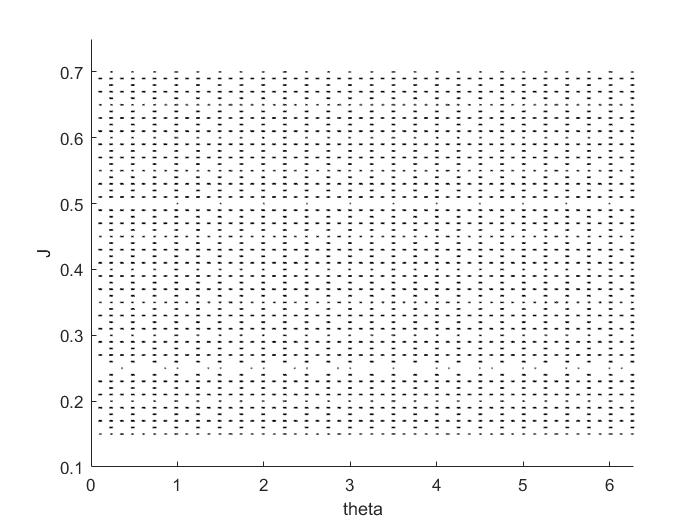
\includegraphics[scale=0.5]{Hamiltonian_1/numerical/figs/Q5_0.0_3646}
		\caption{$V_1=0,V_2=0$ and we see that J is a constant of motion.}
		\label{fig2.1}	
	\end{figure}\newpage
%
%
Now, we increase control values of the perturbations to $V_1=V_2=10^{-4}$ and we obtain (\ref{fig2.2}) \footnote{The different colors correspond to different initial conditions for $\theta$.}
	\begin{figure}[h!]
		\centering 
		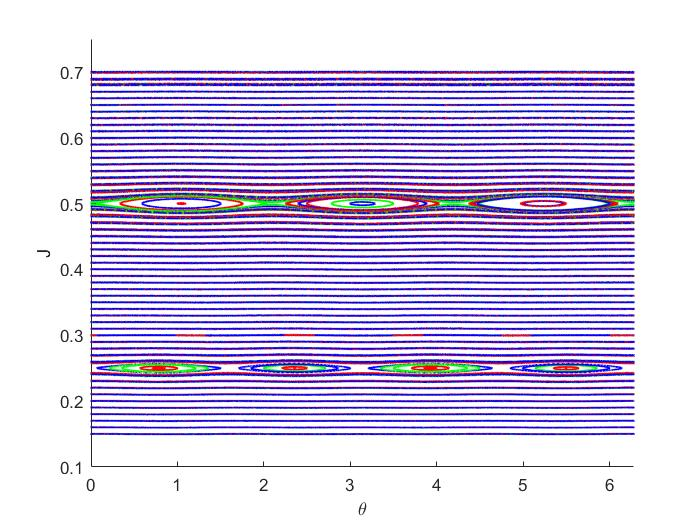
\includegraphics[scale=0.5]{Hamiltonian_1/numerical/figs/Q5_1e-4.1e-4_3634}
		\caption{$V_1=V_2=10^{-4}$ we see that the resonance island emerge at the theoretically expected values of Action}
		\label{fig2.2}
	\end{figure}\\
	
If we further increase the perturbations to $V_1=10^{-3},V_2=10^{-4}$ and $V_1=10^{-4},V_2=10^{-3}$ we have (Figure \ref{fig2.3}), where we see that the islands that correspond to the bigger $V_i$ are larger.\\
%
\begin{figure}[h!]
	\centering
	\begin{subfigure}{.5\textwidth}
  		%\centering
  		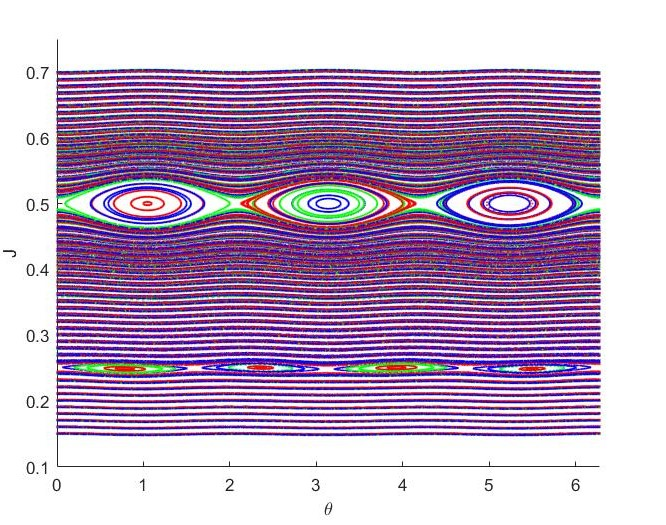
\includegraphics[scale=0.5,left]{Hamiltonian_1/numerical/figs/Q5_1e-3.1e-4_3634}
  		\caption{$V_1=10^{-3},V_2=10^{-4}$}
  		\label{fig2.3a}
	\end{subfigure}%
	\begin{subfigure}{.5\textwidth}
  		%\centering
  		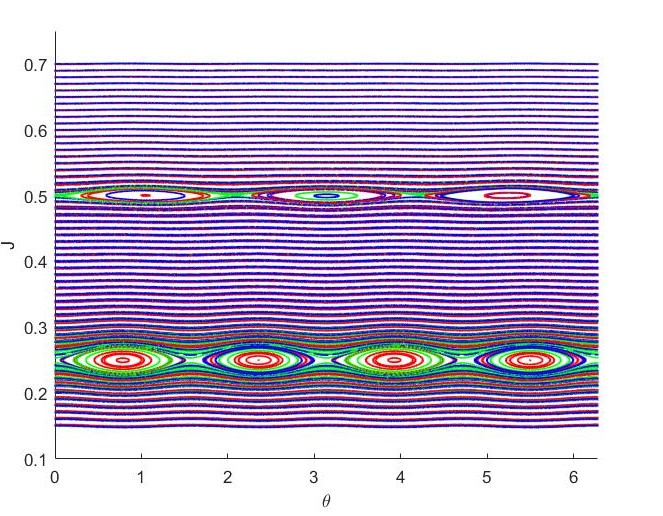
\includegraphics[scale=0.5,right]{Hamiltonian_1/numerical/figs/Q5_1e-4.1e-3_3634}
  		\caption{$V_1=10^{-4},V_2=10^{-3}$}
  		\label{fig2.3b}
	\end{subfigure}
	\caption{Larger $V_i$ corresponds to larger resonance island.}
	\label{fig2.3}
\end{figure}
	%
\begin{figure}[h!]
	\centering
	\begin{subfigure}{.5\textwidth}
  		%\centering
  		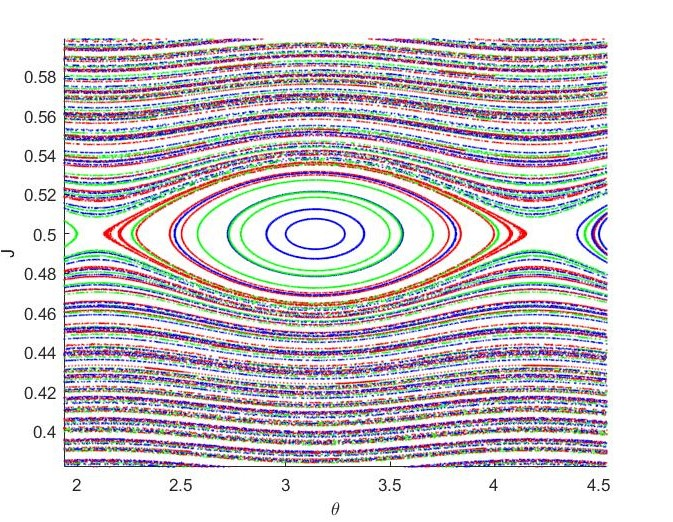
\includegraphics[scale=0.5,left]{Hamiltonian_1/numerical/figs/Q5_1e-3.1e-4_3634_zoom}
  		\caption{$V_1=10^{-3},V_2=10^{-4}$, upper-large islands}
  		\label{fig2.4a}
	\end{subfigure}%
	\begin{subfigure}{.5\textwidth}
  		%\centering
  		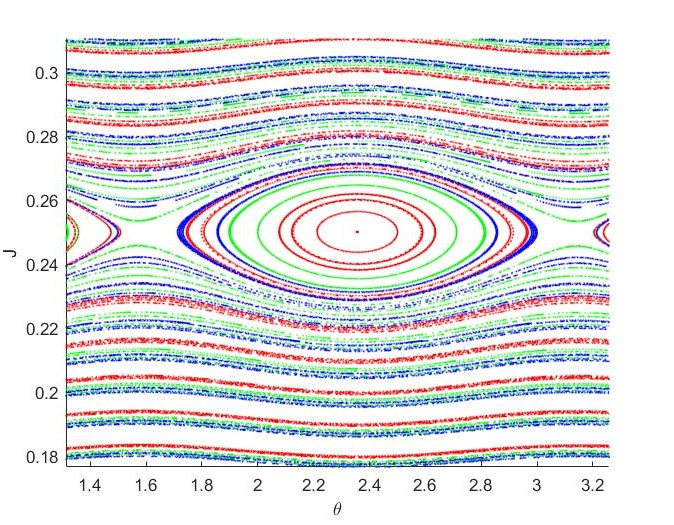
\includegraphics[scale=0.5,right]{Hamiltonian_1/numerical/figs/Q5_1e-4.1e-3_3634_zoom}
  		\caption{$V_1=10^{-4},V_2=10^{-3}$, lower-large islands}
  		\label{fig2.4b}
	\end{subfigure}
	\caption{(Zoomed (Figure \ref{fig2.3})) We see that the islands that correspond to the larger perturbation also have the same width $\Delta J\simeq 0.04$}
	\label{fig2.4}
\end{figure}	\newpage
%
As we increase the value of the perturbations to $V_1=V_2=10^{-3}$ the islands grow larger 
	\begin{figure}[h!]
		\centering
		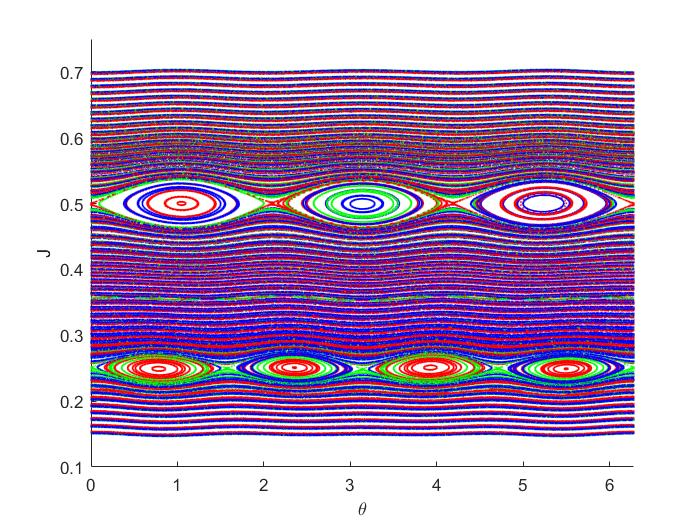
\includegraphics[scale=0.5]{Hamiltonian_1/numerical/figs/Q5_1e-3.1e-3_3634}
		\label{fig2.5}
		\caption{$V_1=V_2=10^{-3}$}
	\end{figure}\\
	%
	Now if we set $V_1=10^{-2}, V_2=10^{-3}$ and $V_1=10^{-3},V_2=10^{-2}$, we see in (Figure (\ref{fig2.6}) that the phase space around the larger perturbation is heavily distorted. 
	%
\begin{figure}[H]
	\centering
	\begin{subfigure}{.5\textwidth}
  		\centering
  		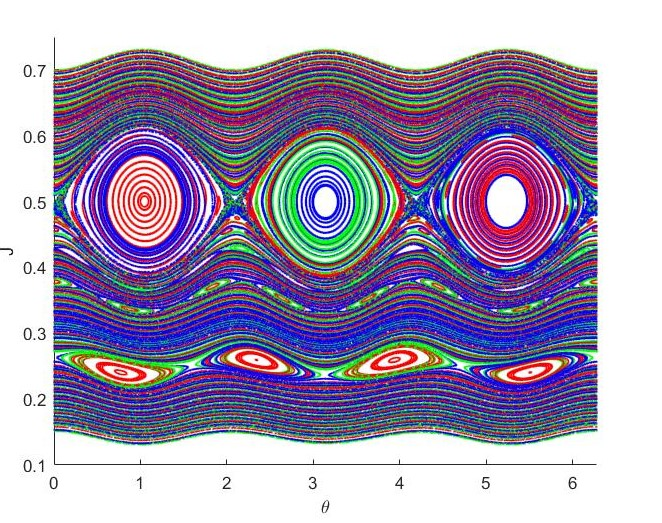
\includegraphics[scale=0.5,left]{Hamiltonian_1/numerical/figs/Q5_1e-2.1e-3_3634}
  		\caption{$V_1=10^{-2},V_2=10^{-3}$, upper-large islands}
  		\label{fig2.6a}
	\end{subfigure}%
	\begin{subfigure}{.5\textwidth}
  		%\centering
  		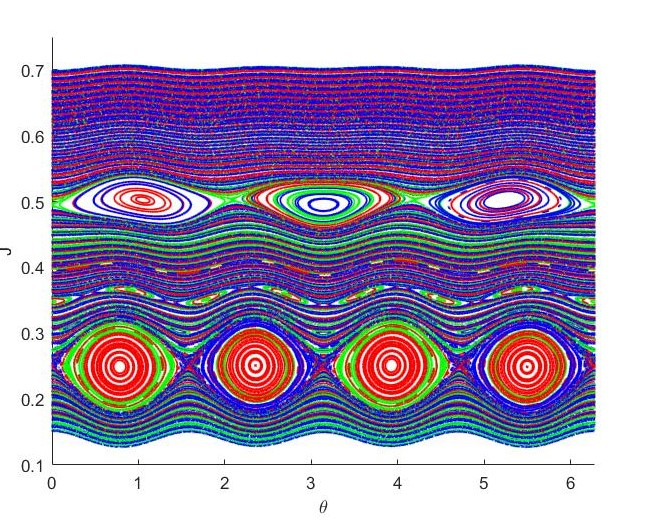
\includegraphics[scale=0.5,right]{Hamiltonian_1/numerical/figs/Q5_1e-3.1e-2_3634}
  		\caption{$V_1=10^{-3},V_2=10^{-2}$, lower-large islands}
  		\label{fig2.6b}
	\end{subfigure}
	\caption{ Again we see that bigger $V_i$ corresponds to larger islands}
	\label{fig2.6}
\end{figure}
%
%zoomed 2.6
\begin{figure}[H]
	\centering
	\begin{subfigure}{.5\textwidth}
  		%\centering
  		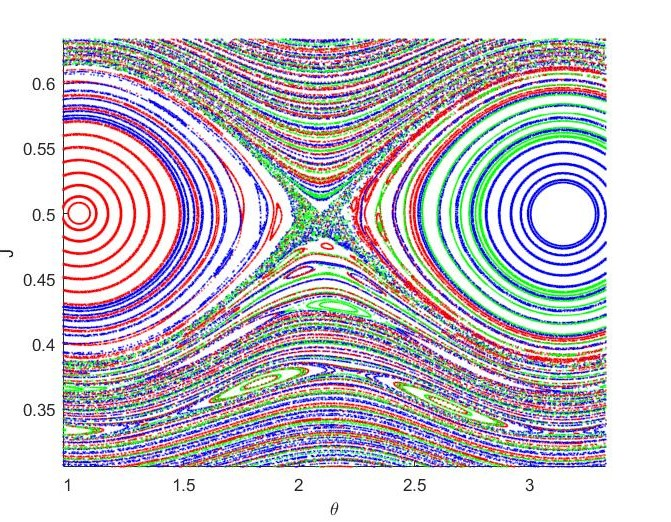
\includegraphics[scale=0.47,left]{Hamiltonian_1/numerical/figs/Q5_1e-2.1e-3_3634_zoom1}
  		\caption{$V_1=10^{-2},V_2=10^{-3}$, upper-large islands}
  		\label{fig2.7a}
	\end{subfigure}%
	\begin{subfigure}{.5\textwidth}
  		%\centering
  		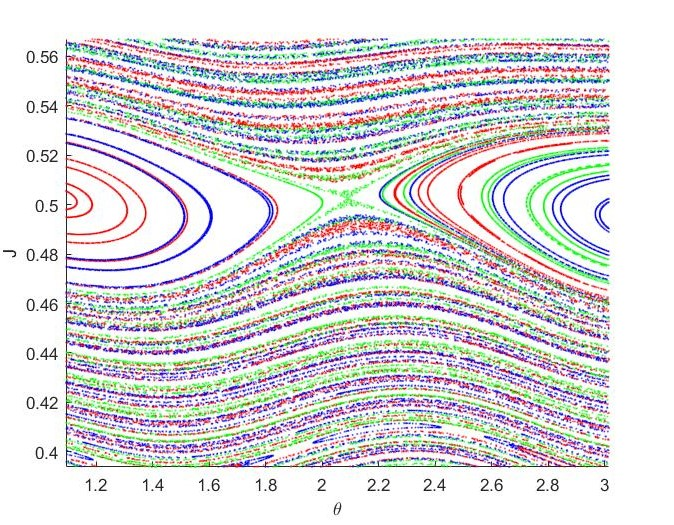
\includegraphics[scale=0.47,right]{Hamiltonian_1/numerical/figs/Q5_1e-3.1e-2_3634_zoom1}
  		\caption{$V_1=10^{-3},V_2=10^{-2}$, lower-large islands}
  		\label{fig2.7b}
	\end{subfigure}
	        %\vskip\baselineskip
	\begin{subfigure}{.49\textwidth}
  		%\centering
  		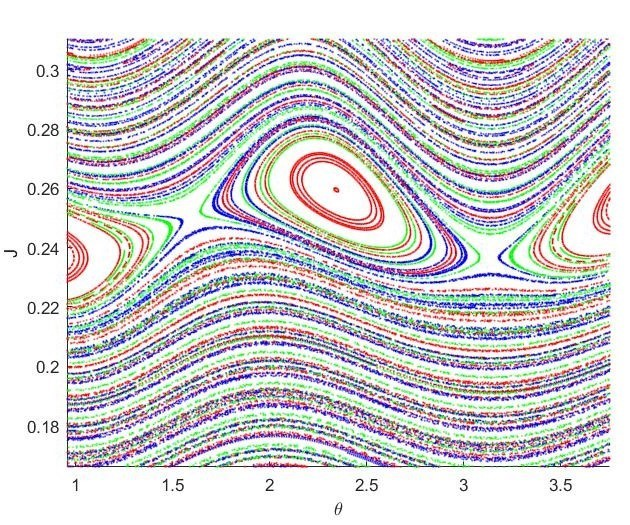
\includegraphics[scale=0.47,left]{Hamiltonian_1/numerical/figs/Q5_1e-2.1e-3_3634_zoom2}
  		\caption{$V_1=10^{-3},V_2=10^{-2}$, lower-large islands}
  		\label{fig2.7c}
	\end{subfigure}
	\begin{subfigure}{.49\textwidth}
  		%\centering
  		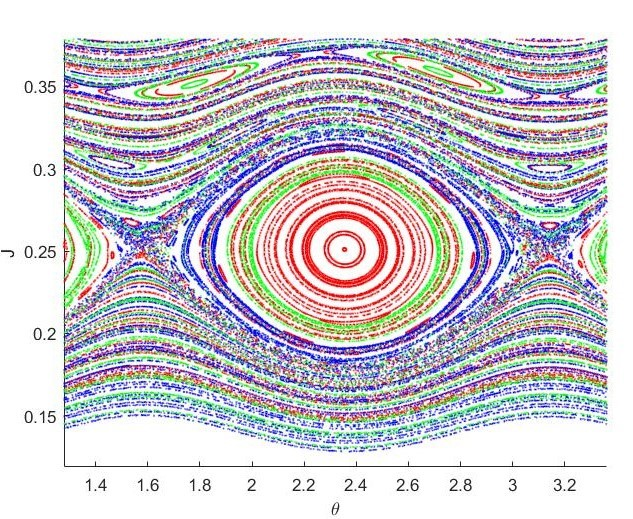
\includegraphics[scale=0.47,right]{Hamiltonian_1/numerical/figs/Q5_1e-3.1e-2_3634_zoom2}
  		\caption{$V_1=10^{-3},V_2=10^{-2}$, lower-large islands}
  		\label{fig2.7d}
	\end{subfigure}
	\caption{(Zoomed (Figure \ref{fig2.6})) We see that the islands that correspond to the larger perturbation also have the same width $\Delta J\simeq 0.04$}
	\label{fig2.7}
\end{figure}
Now, we set both $V_1=V_2=10^{-2}$ and we have (Figure \ref{fig2.8}). As we seem the two separatrices overlap and we have extended chaos.
%
\begin{figure}[H]
	\centering
	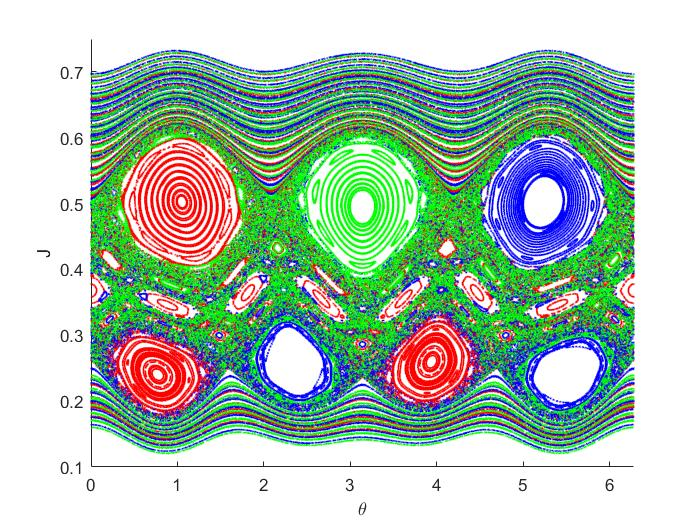
\includegraphics[scale=0.6]{Hamiltonian_1/numerical/figs/Q5_1e-2.1e-2_3634}
	\caption{$V_1=V_2=10^{-2}$}
	\label{fig2.8}
\end{figure}
%x
\begin{figure}[H]
	\centering
	\begin{subfigure}{.32\textwidth}
  		\centering
  		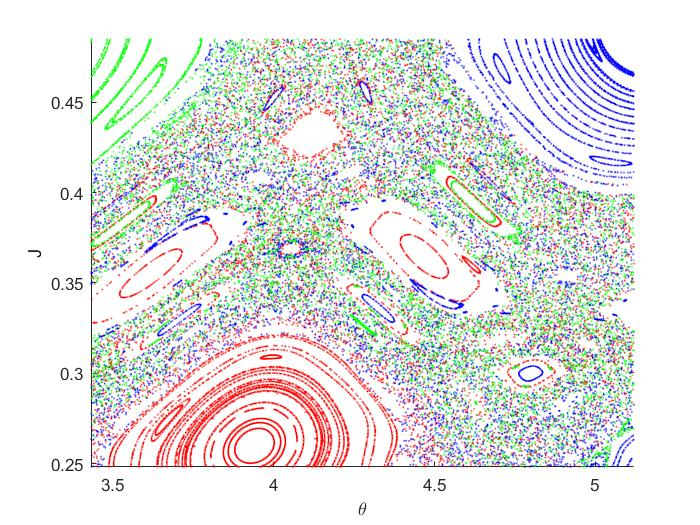
\includegraphics[scale=0.25]{Hamiltonian_1/numerical/figs/Q5_1e-2.1e-2_3634_zoom1}
  		%\caption{$V_1=10^{-2},V_2=10^{-2}$, upper-large islands}
  		\caption{}
  		\label{fig2.9a}
	\end{subfigure}%
	\begin{subfigure}{.32\textwidth}
  		\centering
  		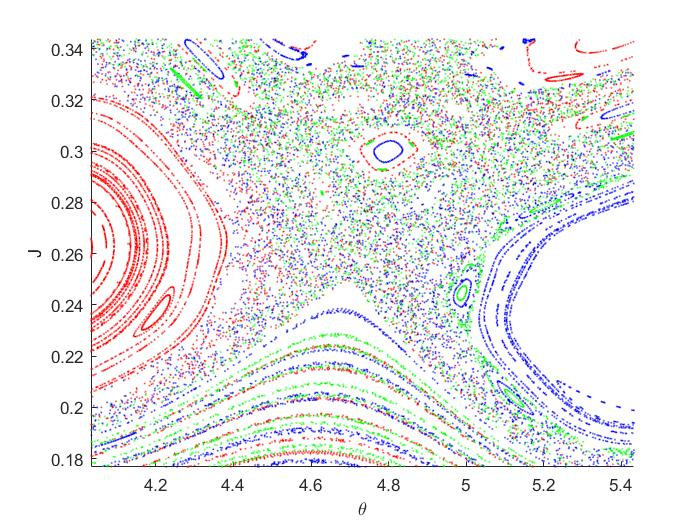
\includegraphics[scale=0.25]{Hamiltonian_1/numerical/figs/Q5_1e-2.1e-2_3634_zoom2}
  		%\caption{$V_1=10^{-2},V_2=10^{-2}$, lower-large islands}
  		\caption{}
  		\label{fig2.9b}
	\end{subfigure}
	%
	\begin{subfigure}{.32\textwidth}
		\centering
		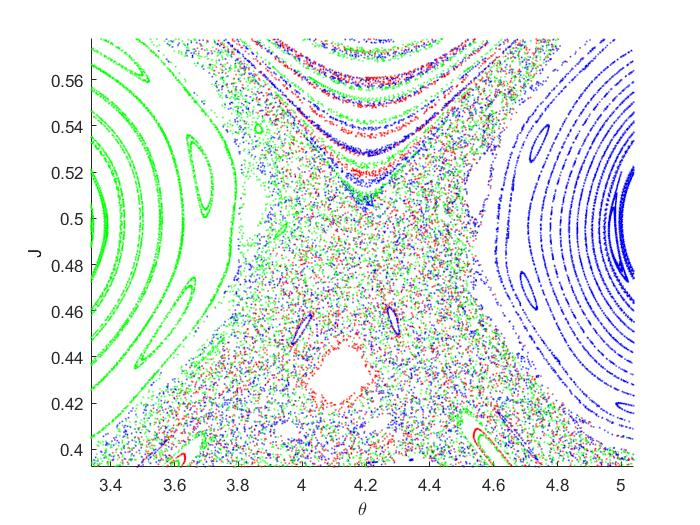
\includegraphics[scale=0.25]{Hamiltonian_1/numerical/figs/Q5_1e-2.1e-2_3634_zoom3}
		\caption{}
		\label{fig2.9c}
	\end{subfigure}
	\label{fig2.9}
	\caption{Zoom in (Figure \ref{fig2.8})}
\end{figure}
%
%%

We can make another remark on the above diagrams. From [1], we have that the width of the resonance islands, that is the distance between the two separatrices, is given by the relation 
	\begin{align*}\label{eq2.22}
		\Delta J_{i,max}= 2n_i \left( \frac{2V_i}{G}\right)^{1/2}
	\end{align*}
	where $G=n_i^2\partial^2(H_0)/\partial^2(J_i)$.
So, for various values of $V_1,V_2$, we have the following values 
\newpage
	\begin{table}[th]
		\centering 
		\begin{tabular}{c|c||c|c}
			$V_1$ & $\Delta J_{1,max}$ & $V_2$ & $\Delta J_{2,max}$ \\ 
			\hline\hline
			$10^{-4}$ & 0.0200& $10^{-4}$ & 0.0200 \\ 
			$10^{-3}$ & 0.0632& $10^{-3}$ & 0.0632 \\
			$10^{-2}$ & 0.2000& $10^{-2}$ & 0.2000 
		\end{tabular}
		\caption{}
		\label{tab2.1}
	\end{table}
	We can notice that for $V_1=V_2=10^{-2}$ the resonace islands overlap which is something that we have already found from the numerical results (Figure \ref{fig2.8}).
	In order to compare the above results with the numerical ones, we use the same code as before, but we restrict the Poincare sections only at a fraction of the phase space near the resonances. In that way we can approximate the separatrices and compare their distance with the values of the Table (\ref{tab2.1}).
\begin{figure}[hb!]
	\centering
	\begin{subfigure}{.49\textwidth}
  		%\centering
  		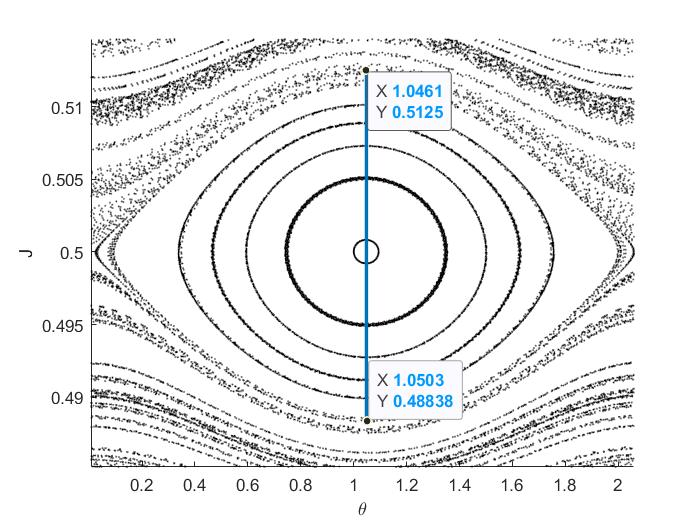
\includegraphics[scale=0.3,left]{Hamiltonian_1/numerical/figs/Q5_dj_1e-4_res1}
  		\caption{$V_1=V_2=10^{-4}$, $J_{res,1}=0.5$ with \\$\Delta J_{1,res}=0.024$}
  		\label{fig2.10a}
	\end{subfigure}%
	\begin{subfigure}{.5\textwidth}
  		%\centering
  		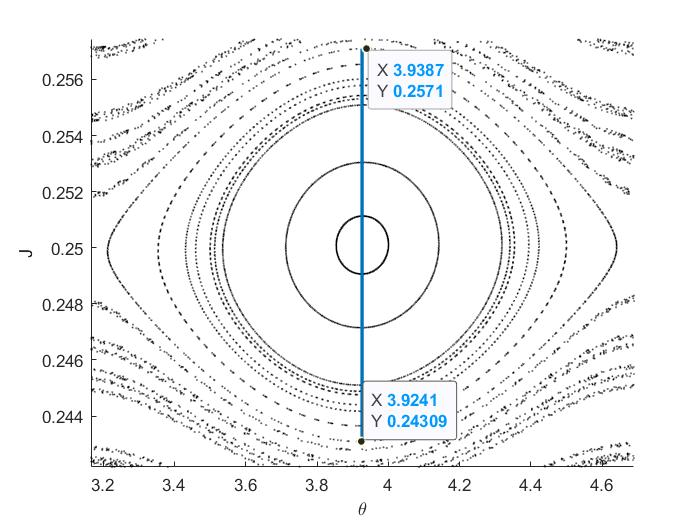
\includegraphics[scale=0.3,right]{Hamiltonian_1/numerical/figs/Q5_dj_1e-4_res2}
  		\caption{$V_1=V_2=10^{-4}$, $J_{res,2}=0.25$ with \\$\Delta J_{2,res}=0.14$}
  		\label{fig2.10b}
	\end{subfigure}%
	        %\vskip\baselineskip
	        \\
	\begin{subfigure}{.49\textwidth}
  		%\centering
  		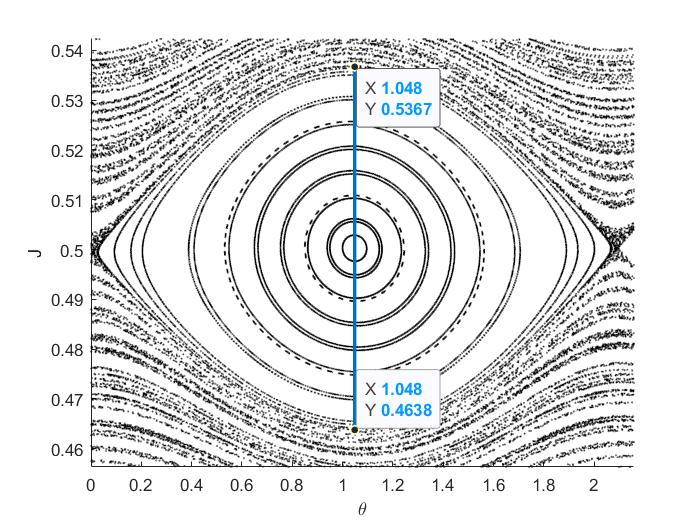
\includegraphics[scale=0.3,left]{Hamiltonian_1/numerical/figs/Q5_dj_1e-3_res1}
  		\caption{$V_1=V_2=10^{-3}$, $J_{res,1}=0.5$ with \\$\Delta J_{1,res}=0.073$}
  		\label{fig2.10c}
	\end{subfigure}
	%
	\begin{subfigure}{.49\textwidth}
  		%\centering
  		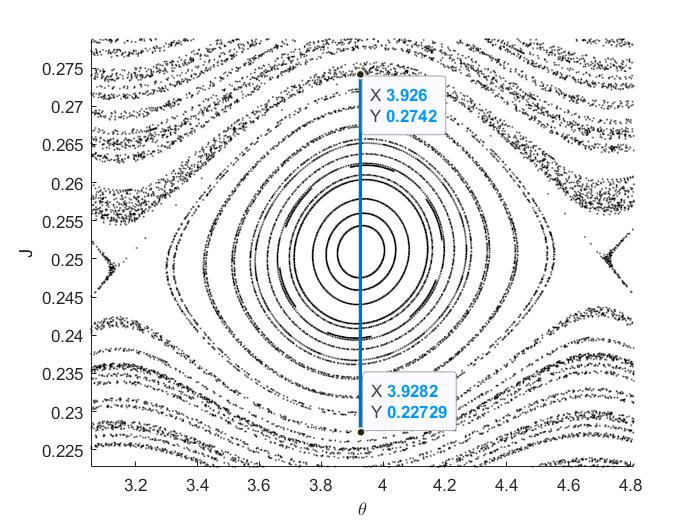
\includegraphics[scale=0.3,right]{Hamiltonian_1/numerical/figs/Q5_dj_1e-3_res2}
  		\caption{$V_1=V_2=10^{-3}$, $J_{res,2}=0.25$ with \\$\Delta J_{2,res}=0.044$}
  		\label{fig2.10d}
	\end{subfigure}	
	%
%	\begin{subfigure}{.49\textwidth}
%  		%\centering
%  		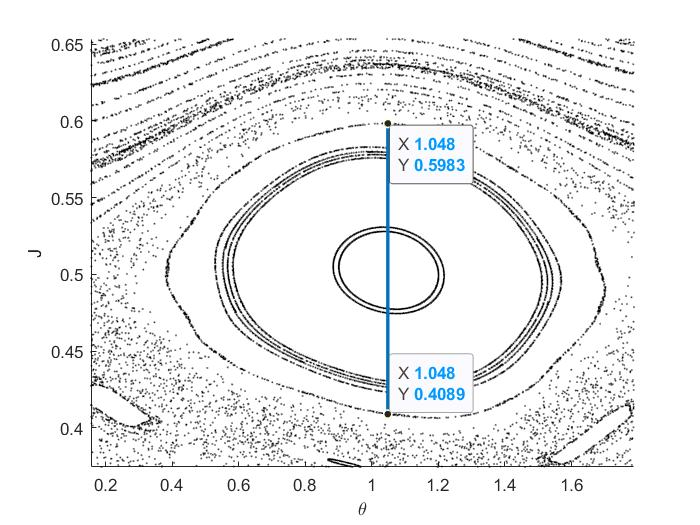
\includegraphics[scale=0.3,left]{Hamiltonian_1/numerical/figs/Q5_dj_1e-2_res1}
%  		\caption{$V_1=V_2=10^{-2}$, $J_{res,1}=0.5$ with $\Delta J_{1,res}=$}
%  		\label{fig2.10e}
%	\end{subfigure}
%	\begin{subfigure}{.49\textwidth}
%  		%\centering
%  		\includegraphics[scale=0.3,right]{Hamiltonian_1/numerical/figs/Q5_dj_1e-2_res2}
%  		\caption{$V_1=V_2=10^{-2}$, $J_{res,2}=0.5$ with $\Delta J_{2,res}=$}
%  		\label{fig2.10f}
%	\end{subfigure}	
	\caption{Poincare Sections to approcimate $\Delta J_{i,res}$ from the numerical results}
	\label{fig2.10}
\end{figure}\\
There analytical and numerical results are relatively close. There are no plots for $V_i=10^{-2}$ since the resonance regions overlap and there are no clear limits of the separatrices.
%==========================================================================
\section*{References}
\begin{itemize}
	\item[[1]] A.J. Lichtenberg \& M.A. Lieberman, Regular and Chaotic Dynamics (2nd edition), Springer 1991
	\item[[2]] H. Goldstein, C. P. Poole, J. Safko, Classical Mechanics (3rd edition), Pearson
	\item[[3]] J. V. Jose, E. J. Saletan, Classical Dyanamics, Cambridge University Press
	\item[[4]] Σ. Ιχτιαρογλου, Εισαγωγή στην Μηχανική Hamilton
\end{itemize}
\end{document}
